\documentclass[12pt,final,fleqn]{article}

% basic packages
\usepackage[margin=1in] { geometry }
\usepackage{amssymb,amsmath, bm}
\usepackage{verbatim}
\usepackage[latin1]{inputenc}
%\usepackage[OT1]{fontenc}
\usepackage{setspace}
\usepackage{enumitem}
\usepackage{url}
\usepackage[font={bf}]{caption}
\usepackage{float}
%\usepackage{pgfplots}
%\usepackage[font={bf}]{caption}
\usepackage{setspace}
\usepackage{latexsym}
%\usepackage{euscript}
\usepackage{graphicx}
\usepackage{marvosym}
\usepackage{amsmath} 
\usepackage{authblk}
\usepackage{xcolor}
%\usepackage[varg]{txfonts}  Older version of ``g'' in math.

% bibliography packages
\usepackage[natbibapa]{apacite}
\bibliographystyle{apacite}
\bibpunct{(}{)}{;}{a}{}{,}
\renewcommand{\bibname}{References}

% hyperref options
\usepackage{color}
\usepackage{hyperref}
\usepackage{xcolor}
\hypersetup{
    colorlinks,
    linkcolor={blue!50!black},
    citecolor={blue!50!black},
    urlcolor={blue!80!black}
}
\newcommand*{\Appendixautorefname}{Appendix}
\renewcommand*{\sectionautorefname}{Section}
\renewcommand*{\subsectionautorefname}{Section}
\newcommand{\aref}[1]{\hyperref[#1]{Appendix~\ref{#1}}}

% packages for tables
\usepackage{longtable}
\usepackage{booktabs, threeparttable}
\usepackage{threeparttablex}
%\usepackage{tabularx}
% dcolumn package
\usepackage{dcolumn}
\newcolumntype{.}{D{.}{.}{-1}}
\newcolumntype{d}[1]{D{.}{.}{#1}}
\captionsetup{belowskip=10pt,aboveskip=-5pt}
\usepackage{multirow}
% rotating package
\usepackage[figuresright]{rotating}
\usepackage{pdflscape}
\usepackage{subcaption}

% packages for figures
\usepackage{grffile}
\usepackage{afterpage}
\usepackage{float}
\usepackage[section]{placeins}


% theorem package
\usepackage{theorem}
\theoremstyle{plain}
\theoremheaderfont{\scshape}
\newtheorem{hyp}{Hypothesis}
\newtheorem{theorem}{Theorem}
\newtheorem{algorithm}{Algorithm}
\newtheorem{assumption}{Assumption}
\newtheorem{lemma}{Lemma}
\newtheorem{proposition}{Proposition}
\newtheorem{remark}{Remark}
\newcommand{\qed}{\hfill \ensuremath{\Box}}
\newcommand\indep{\protect\mathpalette{\protect\independenT}{\perp}}
\DeclareMathOperator{\sgn}{sgn}
\DeclareMathOperator{\tr}{tr}
\DeclareMathOperator{\argmin}{arg\min}
\DeclareMathOperator{\argmax}{arg\max}
\def\independenT#1#2{\mathrel{\rlap{$#1#2$}\mkern2mu{#1#2}}}
\providecommand{\norm}[1]{\lVert#1\rVert}
\renewcommand\r{\right}
\renewcommand\l{\left}
\newcommand\E{\mathbb{E}}
\newcommand\dist{\buildrel\rm d\over\sim}
\newcommand\iid{\stackrel{\rm i.i.d.}{\sim}}
\newcommand\ind{\stackrel{\rm indep.}{\sim}}
\newcommand\cov{{\rm Cov}}
\newcommand\var{{\rm Var}}
\newcommand\SD{{\rm SD}}
\newcommand\bone{\mathbf{1}}
\newcommand\bzero{\mathbf{0}}

% dotted lines in tables
%\usepackage{arydshln}

\usepackage{pdflscape}

% spacing between sections and subsections
\usepackage[compact]{titlesec}

% times new roman
%\usepackage{times}

% appendix settings
\usepackage[toc,page,header]{appendix}
\renewcommand{\appendixpagename}{\centering Appendices}
\usepackage{chngcntr}
\usepackage{etoolbox}
\usepackage{lipsum}


% file paths and definitions
\makeatletter
\newcommand*\ExpandableInput[1]{\@@input#1 }
\makeatother

\setlength{\mathindent}{1cm}
\allowdisplaybreaks[4]
\doublespacing
%\special{pdf: pagesize width 8.5truein height 11.0truein}

\titleformat{\subsection}
  {\itshape\large}{\thesubsection}{1em}{}

\setcounter{tocdepth}{1}

%--------------------------------------------------------------------------------------
% BEGIN DOCUMENT
%--------------------------------------------------------------------------------------

\begin{document}
\singlespace
\title{\textbf{Ballot initiatives and information processing, an experimental approach \\
(Pre-Analysis Plan)}\vspace{-1ex}\thanks{}}
% Thanks
\author{Ang�le Delevoye\thanks{PhD Student in the Department of Political Science, Yale University. angele.delevoye@yale.edu}\vspace{-1ex}}
\author{Trevor Incerti\thanks{PhD Student in the Department of Political Science, Yale University. trevor.incerti@yale.edu}\vspace{-1ex}}
\affil{\textit{}\vspace{-2.5ex}}
\date{\today}
\maketitle

\begin{abstract}
\noindent
\vspace{10cm}
\end{abstract}

\pagebreak

\doublespace


\section{Introduction} \label{sec:Introduction}

One of the most direct ways in which citizens can produce policy is through pure democratic channels such as citizens initiatives, popular consultation, and ballot initiatives. Ballot initiatives have been hailed as an efficient direct democracy mechanism, providing citizens with a much-needed voice in policy making and politics. Defenders of ballot initiatives claim that they provide a way for citizens to voice their opinions and produce policies with less interference from parties and special interests [CITE]. Others caution against the excesses of direct democracy [CITE]. \citet{rosenbluth2018responsible} argue that decentralization of power to the grass roots level has worsened the quality of policy outputs and decision making in the United States by weakening parties. Doubts about voters' competency are also central to the question of whether ballot initiatives lead to adoption of good policies [CITE]. The need for technical knowledge may be  larger on a ballot initiative than in a traditional partisan election as fewer heuristic cues are available. 

We therefore seek to determine how voters use information when asked to vote directly on a supposedly non-partisan, technical policy proposal placed on a ballot initiative. Are voters able to distinguish between the different levels of information quality and bias that stem from varying sources of information? Relatedly, do ballot initiatives actually lead to less interference from parties and special interests, or are voters equally swayed by partisan and special interests cues as objective policy research? 

We propose a field experiment examining voting outcomes on citizen initiated ballot propositions following randomized treatment of proposition endorsement or opposition by parties, special interest groups, and policy experts during the 2020 California state elections. We seek to test whether citizens acting as policy makers give more credence to high quality policy research versus overtly partisan or biased information (i.e. special interests). In addition, we will replicate our field experiment with a survey experiment using identical subjects, treatments, and outcome measures.

The paper will contribute to the growing literature on the effect of campaign outreach on vote choice. A recent meta-analysis by \citet{kalla2018minimal} suggests that the effect of campaign contact and advertising on voting outcomes is close to zero in general elections. However, effects seem to appear when (i) contact is made close to the election and (ii) in primary and ballot measure campaigns, when partisan cues are not present. However, few experiments exist on ballot initiatives. Ballot initiative experiments to date use a single advocacy group to contact voters with a clear position on the policy proposal. By contrast, we know little about whether the quality and/or source of the information provided changes the efficiency of these messages. More broadly, our experimental design also allows to speak to the debate over whether direct democracy is actually more democratic than representative democracy, or if it suffers from the same elite manipulation that might operate in both domains.
 
 A growing literature also suggests that survey experimental results often do not replicate in the field. For example, the zero effect of campaign contact in \citet{kalla2018minimal} does not replicate in survey experiments, and a recent meta analysis of the effects of providing voters with information about the corrupt actions of politicians shows an approximately zero effect in field experiments versus large negative effects in survey environments. By contrast, we hypothesize that survey experiments should better approximate the context of ballot initiatives as: (1) the vote choices are real ballot propositions rather than hypothetical candidates, and (2) partisan cues are less prevalent in (technical) ballot proposals. Whether our hypothesis is correct or incorrect, we will contribute to the growing understanding of the contexts and questions in which survey experiments replicate or do not replicate in the real world.


\section{Theory} \label{sec:Theory}

\subsection{Science, research and democracy}  \label{sec: democracy}

This project speaks to broader theoretical questions on the functioning of our current democracies, and in particular the potential gaps between reality and the ideals of deliberative democracies. We hope therefore hope to contribute to ongoing discussions within philosophy of science, such as perceptions of research methods and consumption of scientific evidence outside of the academy. \\

[Tensions and relationships between science and democracy]

\subsection{Ballot initiatives and direct democracy}

Direct democracy at the US state-level is extremely prevalent, yet understudied. 31 of 50 states permit referendums of some kind, and 24 permit citizen initiatives \citep{leduc2003politics}. Of these 24 states, California engages in more individual exercises of direct democracy than any other. Over the past two decades California has voted on X ballot initiatives at the statewide level [compare to other states], and the number of ballot initiatives per election has increased rapidly over the same period.

Some scholars view this growth of direct democracy as a positive extension of democratic values [CITE AND ADD MORE- SEE LEDUC, HELENE?].

Others contend that the initiative process in the United States has been captured by special interest groups, directly undermining the increased power ballot initiatives are designed to deliver to citizens [CITE - SEE LEDUC]. This implies that the outcomes of direct democracy are no more democratic than representative democracy, as the same elite manipulation that might operate in both domains. For example, the California initiative process has fostered the development of firms that collect signatures to meet required thresholds, and these firms are typically employed by special interest groups. Our research design allows us to evaluate the special interest capture claim by comparing the efficacy of special interest and partisan messages to those of independent policy analysts. 

Ballot initiatives have also been identified as a source of major policy blunders. One of the most notorious of these blunders is California's Proposition 13 of 1978, which capped annual increases of real property taxes to 2 percent per year and prohibited governments from increasing property taxes without a further referendum. Proposition 13 has been blamed for underfunding of California public schools, contributing to California's housing crisis, and perpetuating income inequality in the state. Proposition 13 was not without its critics at the time of passage, with critics contending that ``Proposition 13 raises serious questions about the feasibility of participatory democracy in a policy area which commonly has been dominated by experts'' \citep{mccaffery1978participatory}. In this context, our experimental design allows us to test whether voters are receptive to expert policy analysis warning of negative consequences of ballot referendum policies. 

\subsection{Current experimental evidence}  \label{sec: contact experiments}

A growing body of literature contends that information provision is relatively unsuccessful at changing actual voting outcomes. The primary conclusion from the Metaketa 1 project---which sought to determine if politicians were rewarded for positive information and punished for negative information---was that ``the overall effect of information [provision] across all studies is quite precisely estimated---and not statistically distinguishable from zero'' \citep{dunning2018metaketa}. \citet{incerti2019corruption} draws a similar conclusion in a meta-analysis of corruption information field experiments, finding no voter punishment of allegedly corrupt politicians across field experiments. In the US context, a meta-analysis by \citet{kalla2018minimal} suggests that the effect of campaign contact and advertising on voting outcomes is close to zero in general elections.

However, \citet{kalla2018minimal} find suggestive evidence that campaign contact produces positive effects on vote choice in ballot measure campaigns (see \autoref{fig: kb_meta}). While their meta-analysis includes 23 experiments, these experiments stem from 5 total projects \citep{arceneaux2005using, arceneaux2010comparing, rogers2015ballot}. In each of these projects, voters were contacted by advocacy groups via canvassing, phone, or mail. The existence of positive treatment effects in the ballot initiative environment begs the question of what kinds of informational campaigns are successful. Does high quality policy research persuade voters, or is partisan or special interest contact more effective? 

%\citep{arceneaux2005using}: advocacy group, advocacy message, door to door canvassing, measured turnout and vote. Cluster design, precinct level.
%
%\citep{arceneaux2010comparing}: advocacy group, message tone (negative vs positive vs control), canvassing, measure turnout and vote. Two stage randomization approach, precinct level with clustering. 
%
%\citep{rogers2015ballot}: advocacy group, statewide mail program in Oregon, measure turnout and vote. 

\begin{figure}[h]
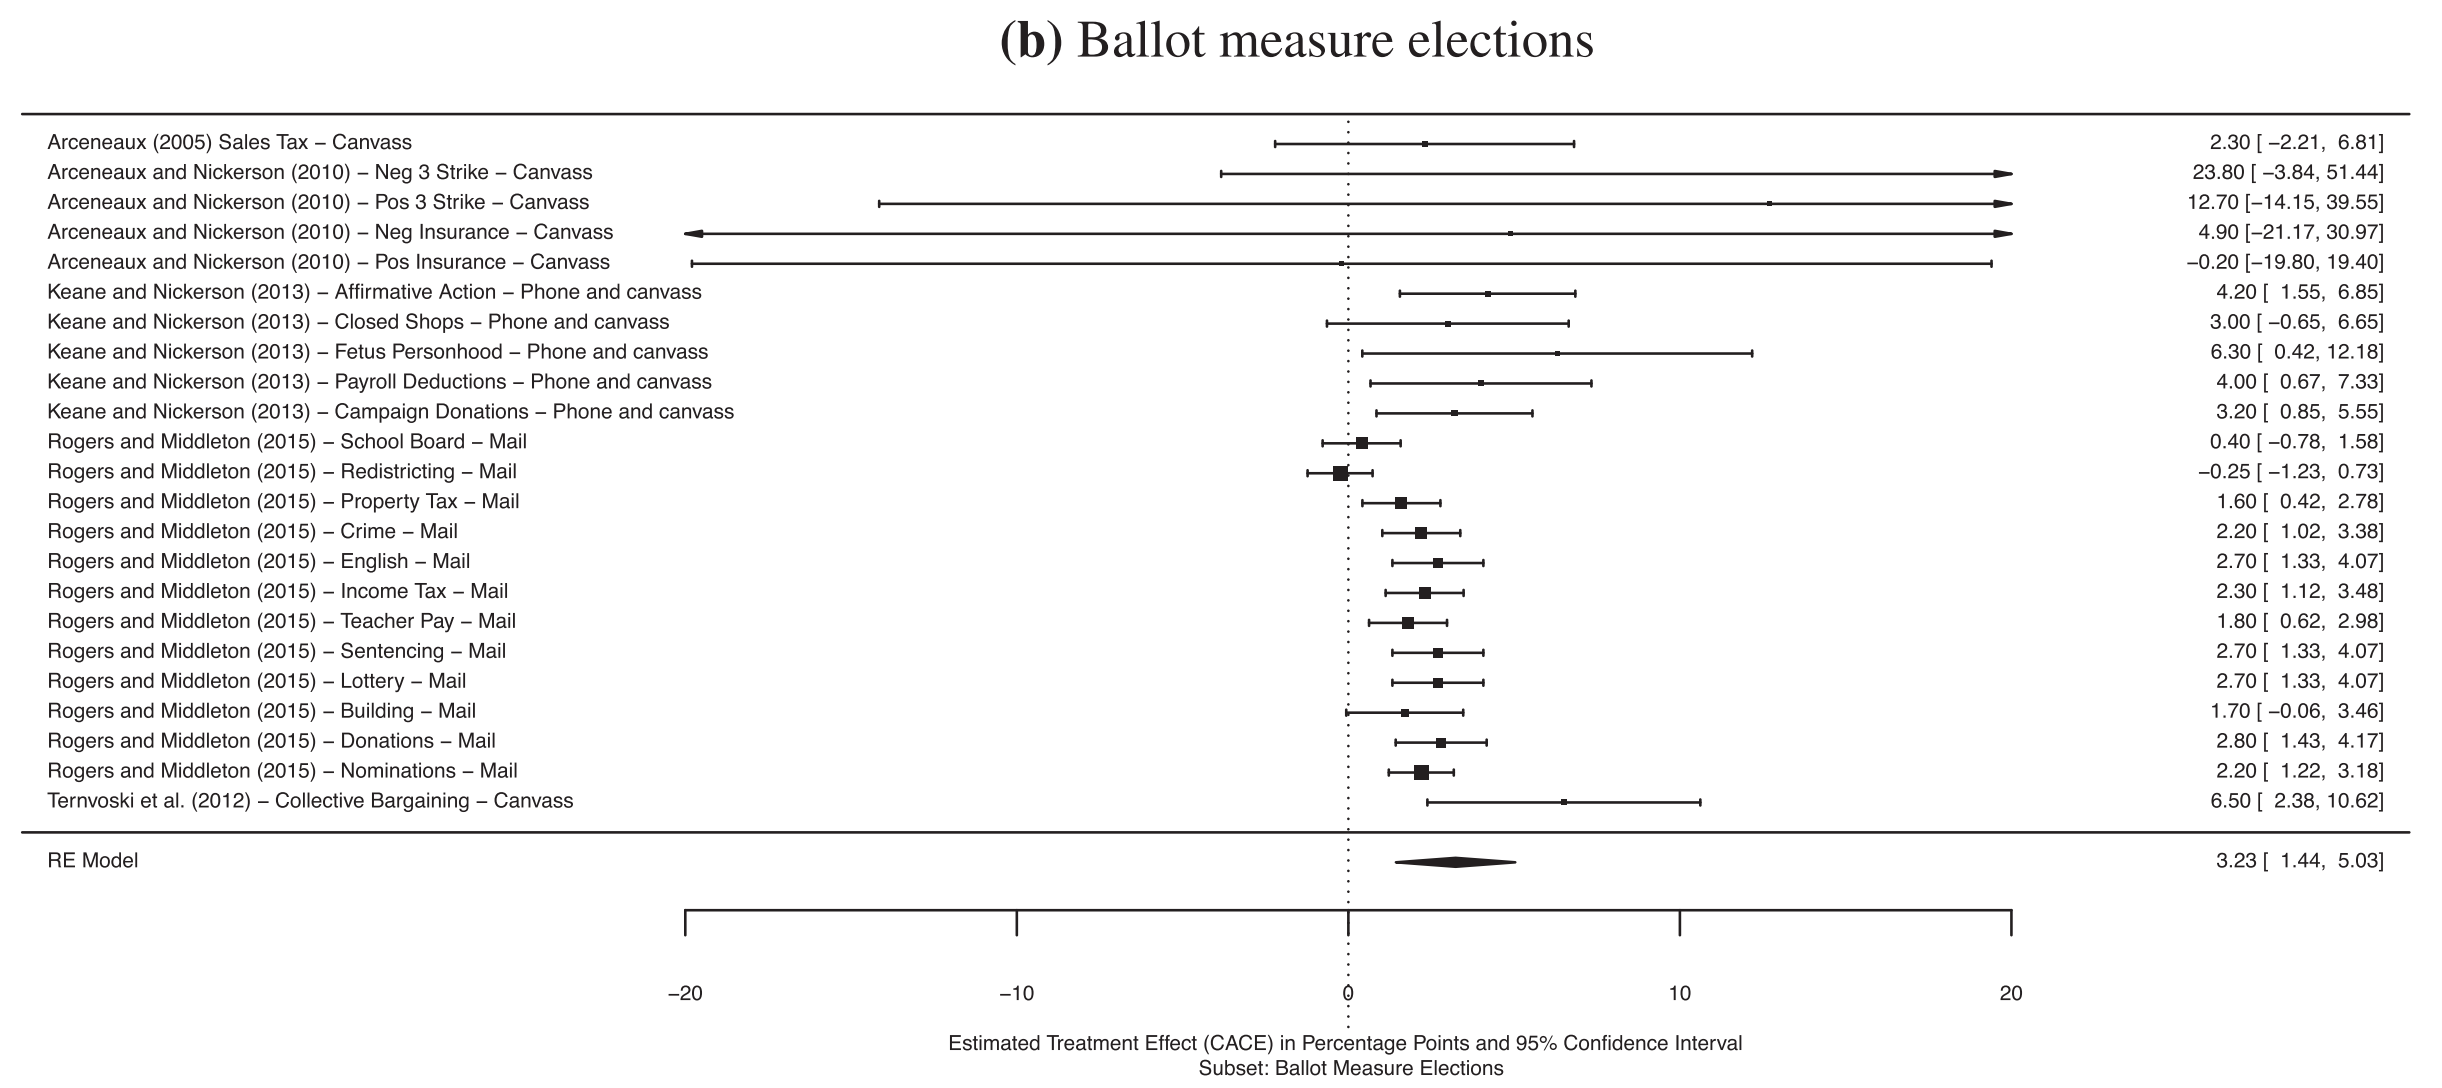
\includegraphics[scale=0.4]{meta_ballot}
\bigbreak
\caption{Meta Analysis on ballot initiatives (from \citet{kalla2018minimal})}
\label{fig: kb_meta}
\end{figure}


\section{Experimental design: field experiment} \label{sec:Design field}

\subsection{Treatment groups and randomization} \label{sec:Treatment}

We would provide voters with different pieces of information leading to a vote on a ballot initiative. This could be different information sources (business vs advocacy group vs academic/scientific), or information vs not information. This information provision could be done through mail (a postcard) or canvassing and phone calls. Postcards: more power, and we would contribute to the literature (postcards don't work in general election campaigns - Kalla Brookman etc, but could they work on a singe, specific policy proposal). Canvassing: less power/geographic reach and probably costlier, but much higher expected treatment effect




\subsection{Outcomes} \label{sec: Outcomes}

Vote on the ballot initiative (at the precinct or smaller level).



\subsection{Choice of policy and election cycles} \label{sec:policy}

Ideal policy: a scientific consensus exists, on a technical subject on which people have very weak priors. Health care, housing, etc. 

Election cycle: off-year vs on-year election. On-year would probably give us access to a lot more voters without strong priors on the specific proposal. 


\section{Experimental design: survey experiment} \label{sec:Design survey}

\subsection{Why do a survey experiment?} \label{sec: questions}

- Methods: field vs survey experiments. Contribute to the growing evidence that survey expeiirments don't give us what we want (campaign reach outs, corruption information, etc). Do it in a very control environment: we would be able to design the syrvey so that it exactly replicates the field. 
- Our priors: survey experiments might be closer to the reality of the real world/a field experiment than in other political contexts. Because technical information, specific proposal with weak priors, no partisan shortcuts, no emotions/feelings involved bc not voting for a person. 
- If right: open the door for more survey experiments, with more ambitious treatments (fake news?). If wrong: survey experiments don't even work in a context where we felt confident that they would. Let's keep building evidence on this. 


\subsection{Design} \label{sec: questions}


\section{Potential natural experiment} \label{sec:natural}

The idea would be to use a real-life variation of information supply. Ex.: data on billboards, with their contents and where exactly they were put on, or a report sent to some precinct but not other. Info provision will probably not be random, so we would need to do a diff and diff (precinct with billboard ? precinct without billboard, but which other difference? Vote on another measure, vote in previous elections, opinion polls on the measure before billboards went up, early voting)? 

\section{Experimental analysis} \label{sec:analysis}

\subsection{Estimation of treatment effects} \label{sec:treatment_effects}

As noted above, we intend to use block random assignment in order  to increase the precision of our treatment effect estimates as well as to facilitate (preregistered) estimation of heterogenous treatment effects. Treatment effect estimates will therefore be calculated as the difference-in-means of the response rate from subjects in each of treatment groups and the response rate from subjects in the control group in each block, weighted by the number of subjects in each block relative to the total number of subjects. More formally, average treatment effects will be estimated as:

\begin{center}
$ATE = \sum_{j = 1}^{J} \frac{N_j}{N}ATE_j$
\end{center}

\noindent
where $J$ is the number of blocks, blocks are indexed by $j$, and $\frac{N_j}{N}$ represents the share of subjects who belong to block $j$. 

In practice, these differences-in-means will be calculated using a weighted least squares regression of response rate on treatment assignment, with weights corresponding to the inverse probability of treatment for each unit (IPW). All p-values will be calculated using randomization inference. As the reference/control group in the experiment is in effect the ``No information / lower tier'' treatment group, all effects must be interpreted in relation to this treatment. In other words, treatment effects should be interpreted as the change in response rate relative to the ``No information / lower tier'' group.

\subsection{Heterogenous treatment effects} \label{sec: hte}


In addition, we will test for heterogenous treatment effects on legislator party and educational attainment. Our test will take the form of regressing our outcome variable on treatments conditional upon the data representing the covariate of interest. In other words, we will split our sample by subject attributes (party and educational attainment), then estimate conditional average treatment effects (CATEs) separately for each of these attributes. For example, to test for heterogenous effects by party, we will regress outcomes on treatments for all legislators in each party. Following estimation of CATEs, we will use randomization inference to test the null hypothesis that CATEs in both groups (e.g. Democrat and Republican) equal to the ATE.

We recognize that the search for heterogenous treatment effects often suffers from the multiple comparisons problem. In a dataset with a large number of covariates, if a large enough number of subgroups is examined, it is highly likely that statistically significant interaction effects will emerge merely by chance. In other words, the more significance tests are performed, the higher the likelihood of falsely rejecting the null hypothesis at least once. We minimize this risk be preregistering our heterogenous effects of interests, as well as by performing multiple comparisons corrections using Bonferroni, Holm-Bonferroni, and Benjamin-Hochburg adjustment procedures.





\section{Conclusion} \label{sec:Conclusion}

Our next steps on this project include finalization of some of the research design decisions that remain open (i.e. federal or state level subjects, partnership with an organization, and choice of the policy). We hope to finalize these details over the summer and to preregister a final Pre-Analysis-Plan with EGAP by the end of 2019. We would then conduct the experiment in 2020. We believe that this timeline would be ideal because of the political and electoral contexts expected in 2020. An election year increases the likelihood that parties will be seeking innovative policy ideas (and decreases the time spent on other legislative activities), and it is therefore possible that legislators will be particularly responsive to information on such policies. 



\clearpage
\pagebreak
\bibliography{bibliography}

\pagebreak

\appendix
\setcounter{table}{0}
\setcounter{figure}{0}
\renewcommand\thetable{\Alph{section}.\arabic{table}}
\renewcommand\thefigure{\Alph{section}.\arabic{figure}}
\section{Appendix} \label{Appendix}





\end{document} 